\chapter{Oscilador caótico utilizando integradores de orden fraccionario}

	\section{Oscilador caótico basado en funciones no lineales saturadas (SNLF)}
	
	Un oscilador caótico basado en funciones no lineales saturadas (SNLF) puede ser descrito por el siguiente sistema de ecuaciones diferenciales:

	\begin{equation} 
		\begin{array}{lcl}
		\dot{x} & = & y \\
		\dot{y} & = & z\\
		\dot{z} & = & -ax - by -cz + hf(x)
		\end{array}
		\label{ec:oscilador_SNLF}
	\end{equation}
	donde  $a, b, c$ y $h$ son coeficientes reales positivas positivos propuestos, con valores en el intervalo $[0, 1]$. $f(x)$ es una función lineal a trozos conocida como deestabilizadora o función saturada
	 
	 El sistema presenta un comportamiento dinámico no lineal gracias a la función saturada desestabilizante $f(x)$. El propósito de dicha función es retroalimentar al sistema y mantenerlo oscilando sin necesidad de una variable de entrada extra en el sistema. Además, esta función desestabilizante es la causante del comportamiento caótico del sistema. La SNLF puede ser descrita mediante una función PWL (PieceWise Linear) cuya forma dependerá del número de enrollamientos requeridos en el sistema caótico.
		
		\section{Función deestabilizadora}
	 El oscilador caótico basado en SNLF descrito en la ecuación (\ref{ec:oscilador_SNLF}) tiene su función saturación expresada como:
	 
	 \begin{equation}
		f(x) = \left\{ \begin{array}{lcl}
		k & \mathrm{si} & x > \beta \\
		sx & \mathrm{si} & - \beta \leq x \leq \beta  \\
		-k & \mathrm{si} & x < -\beta
		\end{array}
		\right.
		\label{ec:saturacion}
	\end{equation}
	donde el parámetro k representa la saturación del sistema, $\beta$ es el punto de quiebre en la función y $s$ es la pendiente entre tramos, en el apéndice \ref{cod:saturation_cust} se muestra una función de MATLAB que realiza esta función. 
	
	Estas funciones pueden generar $n$ cantidad de enrollamientos con la adecuada descripción matemática, en la Figura \ref{fig:Z1_saturacion} se muestra la representación gráfica de la función saturación. 
	
	\begin{figure}[!ht]
		\caption{Función no lineal saturada de dos enrollamientos.} 
		\label{fig:Z1_saturacion}
		\centering
		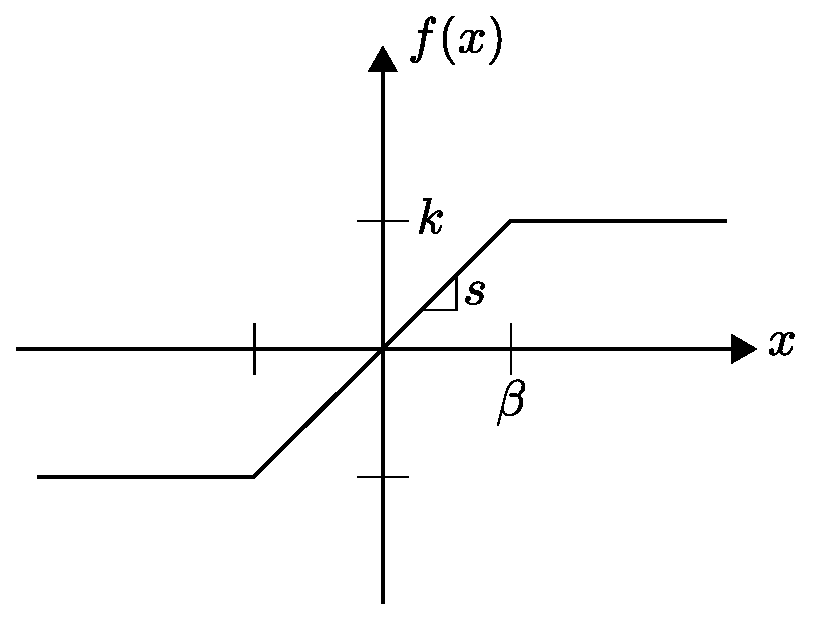
\includegraphics[width=8cm]{Z1_saturacion.eps}
	\end{figure}
	
		\section{Variables de estado del oscilador en orden fraccionario}
	 Para pasar el sistema de la ecuación (\ref{ec:oscilador_SNLF}) a orden fraccionario basta con modificarlo de la siguiente manera:
	 
	 \begin{equation}
		 \begin{array}{lcl}
		_{0}D_{t}^{\alpha}x & = & y \\
		_{0}D_{t}^{\alpha}y  & = & z\\
		_{0}D_{t}^{\alpha}z  & = & -ax - by -cz + hf(x)
		\end{array}
		\label{ec:frac_osc_imp}
	\end{equation}
	
	Las derivadas de orden entero en el sistema de ecuaciones diferenciales acopadas se reemplazan por derivadas de orden fraccionario. El sistema de la ecuación (\ref{ec:frac_osc_imp}) se puede solucionar utilizando el diagrama a bloques de la Figura \ref{fig:Z2_bloques}.
	
	\begin{figure}[!ht]
		\caption{Solución de sistema de orden fraccionario de la ecuación (\ref{ec:frac_osc_imp}).}
		\label{fig:Z2_bloques}
		\centering
		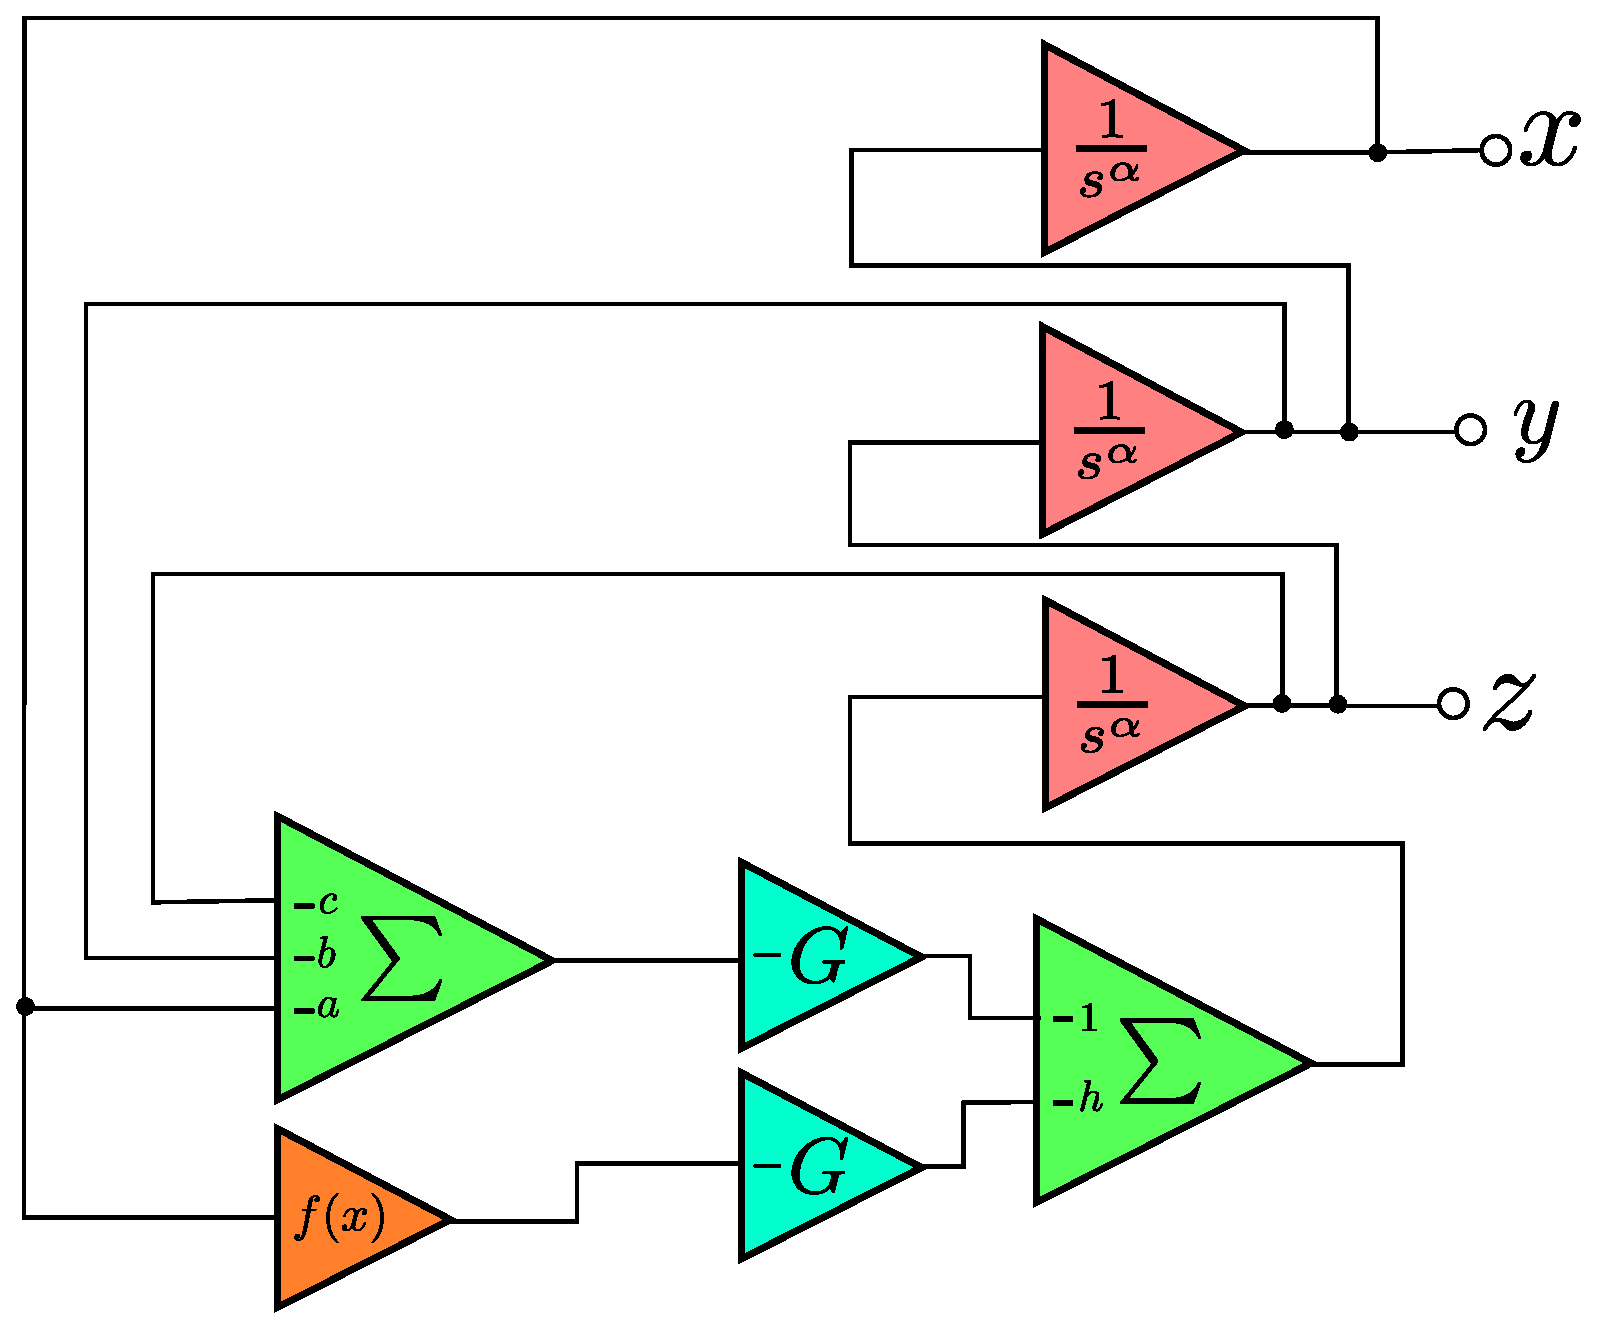
\includegraphics[width=8cm]{Z2_bloques.eps}
	\end{figure}
	
	\section{Implementación en FPAA}
	
	La implementación del oscilador caótico (SNLF) con integradores de orden fraccionario requirió de los 4 FPAA (es necesario colocar los jumpers J8, J9, J10 y ACT1,2,3,4) con los que cuenta la tarjeta. Se optimizó de manera que utilizara la menor cantidad de conexiones externas y se distribuyeron los CAM de modo que fuera sencillo modificar los integradores fraccionarios entre sus distintas aproximaciones o dicho de manera más precisa, entre  sus distintas topologías. 
	
	Para poder realizar las mediciones físicas es necesario utilizar los filtros Rauch que se mencionaron en la sección \ref{sec:rauch} (activar los DIP switches S13 y S12), esto debido a la necesidad de convertir la señal diferencial con que trabaja la FPAA por una single-ended. De mismo modo para interconectar las FPAA es necesario realizar las conexiones físicas sobre la tarjeta, esto se logra activando diversos DIP switches según convenga, en la Tabla \ref{tab:resumen_de_imp} se resumen las conexiones físicas que se tienen que realizar sobre la tarjeta. 
	
	\begin{table}[!ht]                                      
		\centering   
		\caption{Conexiones de DIP switches, jumpers y cables externos.}                            
		\label{tab:resumen_de_imp}                                       
			\begin{tabular}{c c c}                        
			\hline                                              
			Switch & Jumper & Cables externos\\            
			\hline       
			{\color{magenta} S$3$ $\quad2\downarrow$}& J8 & FPAA1 O3 $\rightarrow$ FPAA3 I5\\  
			{\color{magenta} S$5$ $\quad2\downarrow$}& J9& FPAA1 I5 $\rightarrow$ FPAA3 O5\\
			{\color{red} S$4$ $\quad2\uparrow$}&J10&\\ 
			{\color{red} S$6$ $\quad2\uparrow$}&ACT1 &\\
			{\color{blue} S$7$ $\quad2\uparrow$}& ACT2 &\\ 
			S12& ACT3 &\\ 
			S13& ACT4 &\\ 
			\hline                                 
			\end{tabular}                                                             
	\end{table}	
	
	\subsection{Configuración bilineal polo y cero}
	En la Figura \ref{fig:Y1_implementacion} se presenta el diseño final del oscilador caótico (SNLF) implementado en la tarjeta utilizando la configuración bilineal polo y cero con un  orden $\alpha = 0.8$ y con las constantes $a =4$, $b = 0.7$, $c = 0.7$ y $h = 4$. La función de saturación se propuso con los parámetros $k = 2$, $s = 1$ y $\beta= 1.5$ dando como resultado el comportamiento mostrado en la Figura \ref{fig:Z8_saturacion}. Es necesario generar la lookup table utilizando los códigos de los apéndices \ref{cod:saturation_cust} y \ref{cod:D1_Look_up_table}.
	
	\begin{figure}[!ht]
		\caption{Diagrama de implementación en AD2 configuración bilineal polo y cero.} 
		\label{fig:Y1_implementacion}
		\centering
		\includegraphics[width=14cm]{Y1_implementacion.png}
	\end{figure}
	
	Los 4 FPAA se configuraron con las mismas frecuencias de reloj las cuales se muestran en la Figura \ref{fig:Z3_relojes}. Hay que recordar que para $\alpha = 0.8$ los valores para el integrador con aproximación bilineal polo y cero son los siguientes:
	
	\begin{table}[!hbp]                                      
		\centering   
		\caption{Valores para configurar un filtro bilineal como integrador de orden fraccionario con $\alpha = 0.8$.}                            
		\label{tab:respaso}                                        
			\begin{tabular}{ccccc}                        
			\hline                                              
			$\bm{\alpha}$ & $\bm{f_{p}}\,\,$ [kHz] & $\bm{f_{z}}\,\,$ [kHz] & $\bm{G_{L}}$ & $\bm{G_{H}}$ \\            
			\hline                                                                                       
			0.80 & 0.111111 & 9.000000 & 9.000000 & 0.111111 \\  
			\hline                                              
			\end{tabular}                                                                
	\end{table} 
	\begin{figure}[!ht] 
		\caption{Configuración de clocks de todos los FPAA.}
		\label{fig:Z3_relojes}
		\centering
		\includegraphics[width = 12cm]{Z3_relojes.eps}
	\end{figure}
	
	En las Figuras \ref{fig:Z4_FPAA1}, \ref{fig:Z5_FPAA2}, \ref{fig:Z6_FPAA3}, \ref{fig:Z7_FPAA4} se muestran las configuraciones de los CAM desde la FPAA1 hasta la 4.
	\begin{figure}[!ht] 
		\caption{Configuración de los CAM de FPAA1.}
		\label{fig:Z4_FPAA1}
		\centering
		\includegraphics[width = 14cm]{Z4_FPAA1.eps}
	\end{figure}
	
	\begin{figure}[!ht] 
		\caption{Configuración de los CAM de FPAA2.}
		\label{fig:Z5_FPAA2}
		\centering
		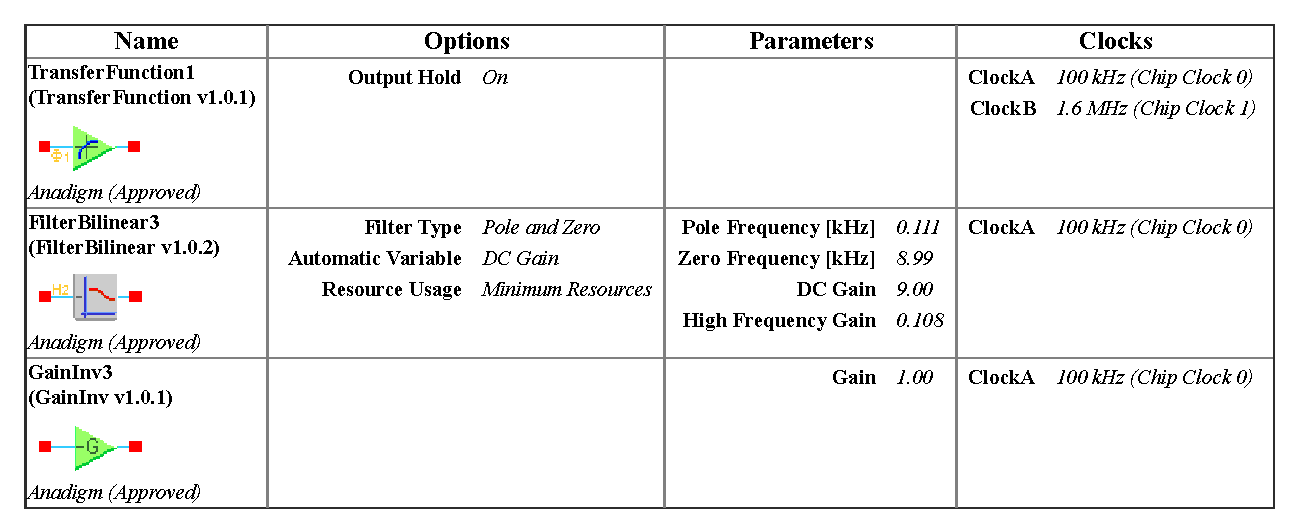
\includegraphics[width = 14cm]{Z5_FPAA2.eps}
	\end{figure}
	
	El comportamiento del oscilador depende directamente de los valores de los parámetros que se eligieron, la función de saturación y el orden fraccionario. Si se modifica ligeramente la función de saturación el sistema pierde su capacidad de oscilar, lo mismo ocurre si se modifica alguno de los parámetros del sistema. 
	
	En las Figuras \ref{fig:fase_imp_osc} y \ref{fig:temporal_imp} se muestran los resultados experimentales. En la primera se muestran los planos de fase o atractores  del sistema y en la segunda la respuesta en el dominio temporal de cada una de estas.
	\begin{figure}[!ht] 
		\caption{Configuración de los CAM de FPAA3.}
		\label{fig:Z6_FPAA3}
		\centering
		\includegraphics[width = 14cm]{Z6_FPAA3.eps}
	\end{figure}
	
	\begin{figure}[!ht] 
		\caption{Configuración de los CAM de FPAA4.}
		\label{fig:Z7_FPAA4}
		\centering
		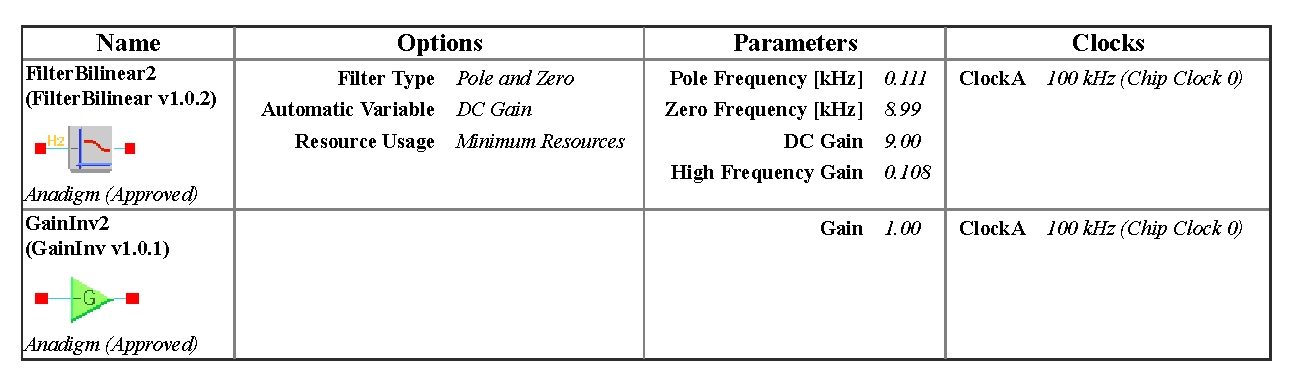
\includegraphics[width = 14cm]{Z7_FPAA4.eps}
	\end{figure}
	
	\begin{figure}[!ht]
		\caption{Función de saturación $k = 2$, $s = 1$ y $\beta= 1.5$.} 
		\label{fig:Z8_saturacion}
		\centering
		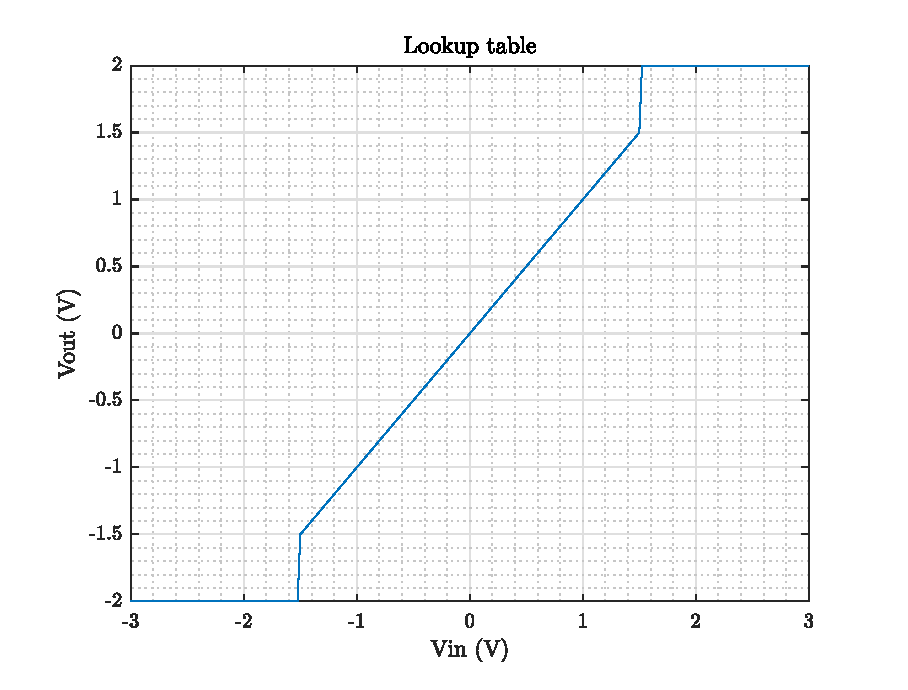
\includegraphics[width=10cm]{Z8_saturacion.eps}
	\end{figure}

	
	\begin{figure}[!ht]
	\caption{Vistas de plano fase del comportamiento del oscilador caótico con $\alpha = 0.8$ y dos enrollamientos.}
	\label{fig:fase_imp_osc}
	  \begin{subfigure}[b]{0.3\textwidth}
	    \includegraphics[trim={6cm 2cm 9cm 2cm},clip,width=\textwidth]{Y2_X_vs_Y.png}
	    \caption{$x$ vs $y$}
	    \label{Y2_X_vs_Y}
	  \end{subfigure}
	  \hfill
	  \begin{subfigure}[b]{0.3\textwidth}
	    \includegraphics[trim={6cm 2cm 9cm 2cm},clip,width=\textwidth]{Y4_X_vs_Z.png}
	    \caption{$x$ vs $z$}
	    \label{fig:Y4_X_vs_Z}
	  \end{subfigure}
	  \hfill
	  \begin{subfigure}[b]{0.3\textwidth}
	    \includegraphics[trim={6cm 2cm 9cm 2cm},clip,width=\textwidth]{Y6_Y_vs_Z.png}
	    \caption{$y$ vs $z$}
	    \label{Y6_Y_vs_Z}
	  \end{subfigure}
	\end{figure}
	
	\begin{figure}[!ht]
	\caption{Respuesta en el dominio temporal de oscilador caótico con $\alpha = 0.8$ y dos enrollamientos.}
	\label{fig:temporal_imp}
	  \begin{subfigure}[b]{0.3\textwidth}
	    \includegraphics[trim={6cm 2cm 9cm 2cm},clip,width=\textwidth]{Y3_X_vs_Y_signal.png}
	    \caption{$x$ vs $y$}
	    \label{fig:Y3_X_vs_Y_signal}
	  \end{subfigure}
	  \hfill
	  \begin{subfigure}[b]{0.3\textwidth}
	    \includegraphics[trim={6cm 2cm 9cm 2cm},clip,width=\textwidth]{Y5_X_vs_Z_signal.png}
	    \caption{$x$ vs $z$}
	    \label{fig:Y5_X_vs_Z_signal}
	  \end{subfigure}
	  \hfill
	  \begin{subfigure}[b]{0.3\textwidth}
	    \includegraphics[trim={6cm 2cm 9cm 2cm},clip,width=\textwidth]{Y7_Y_vs_Z_signal.png}
	    \caption{$y$ vs $z$}
	    \label{fig:Y7_Y_vs_Z_signal}
	  \end{subfigure}
	\end{figure}
	
	\subsection{Configuración bilineal suma de filtros}
	
	En la Figura \ref{fig:Y1p_implementacion} se presenta el diseño final del oscilador caótico (SNLF) implementado en la tarjeta utilizando la configuración bilineal suma de filtros con un  orden $\alpha = 0.9$ y con las constantes $a =4$, $b = 0.7$, $c = 0.7$ y $h = 4$. 
	
	\begin{figure}[!ht]
		\caption{Diagrama de implementación en AD2 configuración bilineal suma de filtros.} 
		\label{fig:Y1p_implementacion}
		\centering
		\includegraphics[width=14cm]{Y1p_implementacion.png}
	\end{figure}
	
	Los 4 FPAA se configuraron con las mismas frecuencias de reloj las cuales se muestran en la Figura \ref{fig:Z3p_relojes}. Hay que recordar que para $\alpha = 0.9$ los valores para el integrador con aproximación bilineal suma de filtros son los siguientes:
	
	\begin{table}[!hbp]                                      
		\centering   
		\caption{Valores para configurar implementación suma de pasabajas y paaltas de ordenes de 0.1 a 0.95.}                            
		\label{tab:repaso2}                                        
			\begin{tabular}{cccc}                        
			\hline                                              
			$\bm{\alpha}$ & $\bm{G_{1}}\,\,$ [LP] & $\bm{G_{2}}\,\,$ [HP] & $\bm{f_{0}}\,\,$ [kHz]  \\            
			\hline                                                                         
			0.90 & 19.000000 & 0.052632 & 0.052632 \\
			\hline                                              
			\end{tabular}                                                                
	\end{table} 	
	
	
	\begin{figure}[!ht] 
		\caption{Configuración de clocks de todos los FPAA.}
		\label{fig:Z3p_relojes}
		\centering
		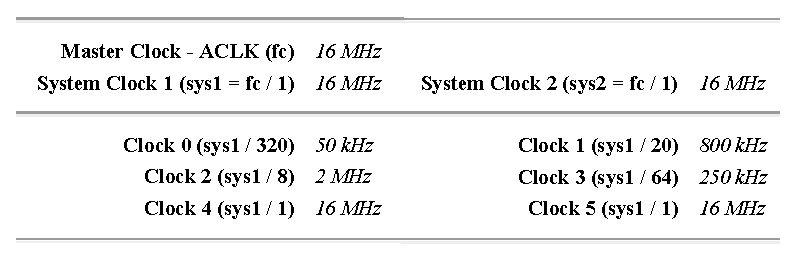
\includegraphics[width = 12cm]{Z3p_relojes.eps}
	\end{figure}
	
	En las Figuras \ref{fig:Z4p_FPAA1}, \ref{fig:Z5p_FPAA2}, \ref{fig:Z6p_FPAA3}, \ref{fig:Z7p_FPAA4} se muestran las configuraciones de los CAM desde la FPAA1 hasta la 4.
	\begin{figure}[!ht] 
		\caption{Configuración de los CAM de FPAA1.}
		\label{fig:Z4p_FPAA1}
		\centering
		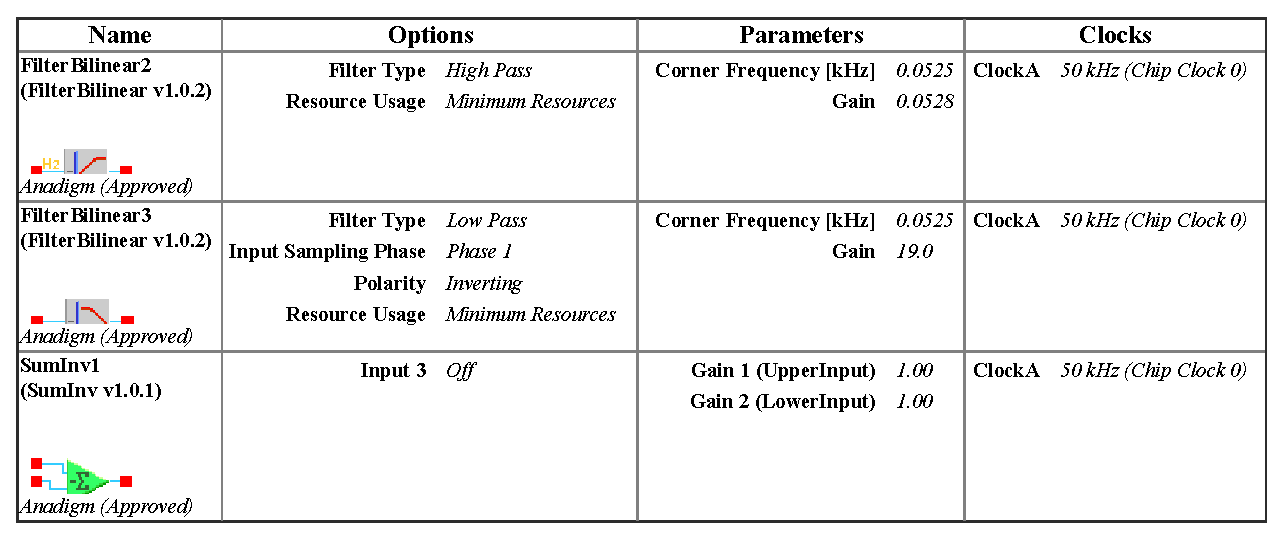
\includegraphics[width = 14cm]{Z4p_FPAA1.eps}
	\end{figure}
	
	\begin{figure}[!ht] 
		\caption{Configuración de los CAM de FPAA2.}
		\label{fig:Z5p_FPAA2}
		\centering
		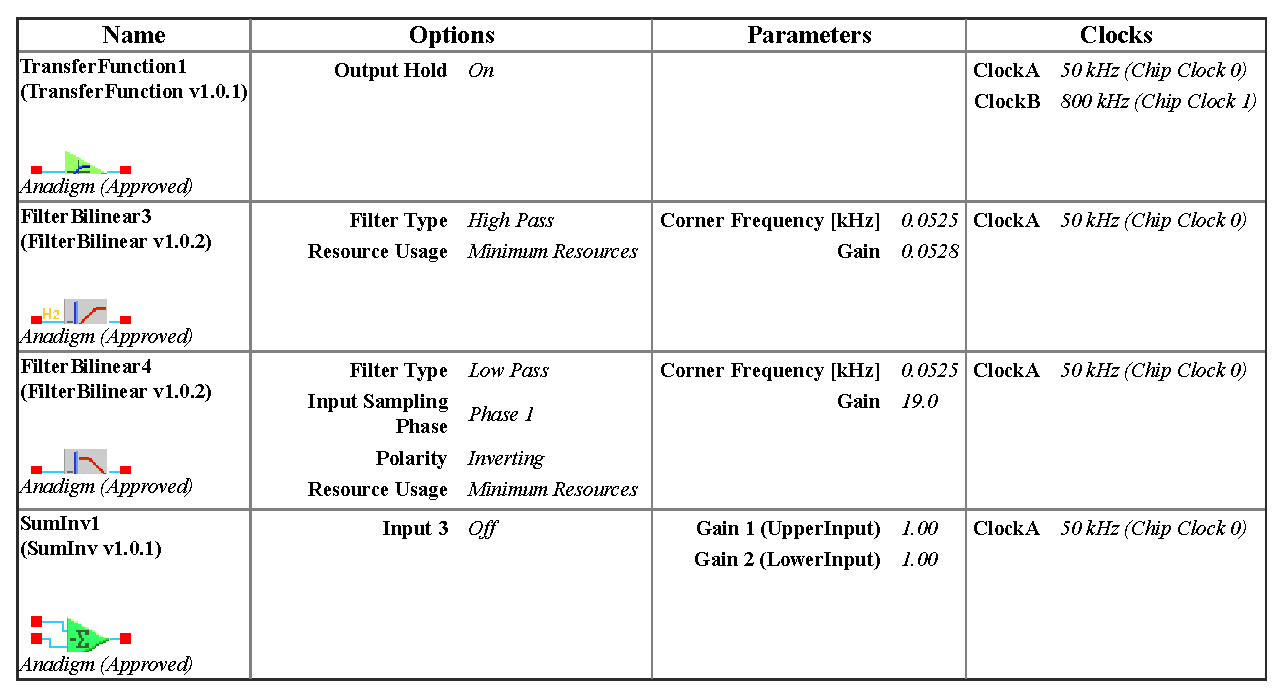
\includegraphics[width = 14cm]{Z5p_FPAA2.eps}
	\end{figure}
	
	En las Figuras \ref{fig:fasep_imp_osc} y \ref{fig:temporalp_imp} se muestran los resultados experimentales. En la primera se muestran los planos de fase o atractores  del sistema y en la segunda la respuesta en el dominio temporal de cada una de estas.
	\begin{figure}[!ht] 
		\caption{Configuración de los CAM de FPAA3.}
		\label{fig:Z6p_FPAA3}
		\centering
		\includegraphics[width = 14cm]{Z6p_FPAA3.eps}
	\end{figure}
	
	\begin{figure}[!ht] 
		\caption{Configuración de los CAM de FPAA4.}
		\label{fig:Z7p_FPAA4}
		\centering
		\includegraphics[width = 14cm]{Z7p_FPAA4.eps}
	\end{figure}
	

	
	\begin{figure}[!ht]
	\caption{Vistas de plano fase del comportamiento del oscilador caótico con $\alpha = 0.8$ y dos enrollamientos.}
	\label{fig:fasep_imp_osc}
	  \begin{subfigure}[b]{0.3\textwidth}
	    \includegraphics[trim={6cm 2cm 9cm 2cm},clip,width=\textwidth]{Y2p_X_vs_Y.png}
	    \caption{$x$ vs $y$}
	    \label{Y2p_X_vs_Y}
	  \end{subfigure}
	  \hfill
	  \begin{subfigure}[b]{0.3\textwidth}
	    \includegraphics[trim={6cm 2cm 9cm 2cm},clip,width=\textwidth]{Y4p_X_vs_Z.png}
	    \caption{$x$ vs $z$}
	    \label{fig:Yp4_X_vs_Z}
	  \end{subfigure}
	  \hfill
	  \begin{subfigure}[b]{0.3\textwidth}
	    \includegraphics[trim={6cm 2cm 9cm 2cm},clip,width=\textwidth]{Y6p_Y_vs_Z.png}
	    \caption{$y$ vs $z$}
	    \label{Y6p_Y_vs_Z}
	  \end{subfigure}
	\end{figure}
	
	\begin{figure}[!ht]
	\caption{Respuesta en el dominio temporal de oscilador caótico con $\alpha = 0.8$ y dos enrollamientos.}
	\label{fig:temporalp_imp}
	  \begin{subfigure}[b]{0.3\textwidth}
	    \includegraphics[trim={6cm 2cm 9cm 2cm},clip,width=\textwidth]{Y3p_X_vs_Y_signal.png}
	    \caption{$x$ vs $y$}
	    \label{fig:Y3p_X_vs_Y_signal}
	  \end{subfigure}
	  \hfill
	  \begin{subfigure}[b]{0.3\textwidth}
	    \includegraphics[trim={6cm 2cm 9cm 2cm},clip,width=\textwidth]{Y5p_X_vs_Z_signal.png}
	    \caption{$x$ vs $z$}
	    \label{fig:Y5p_X_vs_Z_signal}
	  \end{subfigure}
	  \hfill
	  \begin{subfigure}[b]{0.3\textwidth}
	    \includegraphics[trim={6cm 2cm 9cm 2cm},clip,width=\textwidth]{Y7p_Y_vs_Z_signal.png}
	    \caption{$y$ vs $z$}
	    \label{fig:Y7p_Y_vs_Z_signal}
	  \end{subfigure}
	\end{figure}